\documentclass[12pt]{article} % use larger type; default would be 10pt
\usepackage[utf8]{inputenc} % set input encoding (not needed with XeLaTeX)

%%% PAGE DIMENSIONS
\usepackage{geometry} % to change the page dimensions
\geometry{a4paper} % or letterpaper (US) or a5paper or....
\geometry{margin=2cm} % or letterpaper (US) or a5paper or....

\usepackage{graphicx} % support the \includegraphics command and options
\usepackage[parfill]{parskip} % Activate to begin paragraphs with an empty line rather than an indent
\usepackage{times} % for Times Roman default font

%%% PACKAGES
\usepackage{booktabs} % for much better looking tables
\usepackage{array} % for better arrays (eg matrices) in maths
\usepackage{paralist} % very flexible & customisable lists (eg. enumerate/itemize, etc.)
\usepackage{verbatim} % adds environment for commenting out blocks of text & for better verbatim
\usepackage{subfig} % make it possible to include more than one captioned figure/table in a single float

%%% HEADERS & FOOTERS
\usepackage{fancyhdr} % This should be set AFTER setting up the page geometry
\pagestyle{fancy} % options: empty , plain , fancy
\renewcommand{\headrulewidth}{0pt} % customise the layout...
\lhead{}\chead{}\rhead{}
\lfoot{}\cfoot{\thepage}\rfoot{}

\makeatletter
\renewcommand{\maketitle}{%
  {\bfseries{\scshape{\Large{\@title\par}}}}
}
\makeatother

\hyphenation{Kiwi-bank} % otherwise it may get hyphenated as Ki-wibank

%%% END Article customizations

%%% The "real" document content comes below...

\title{Mueller Tarn (camping and high-circ): 12-13 November 2017}

\begin{document}
  \maketitle
We started walking about 14:00, being uncertain of how long the trip would take carrying packs.  However, we were pleasantly surprised to arrive at the camp site within a couple of hours.  There are still parts of the track that could do with more marking.  The camp site at the tarn is idyllic with a separate spot for the tent and one for the fire (there is also an alternative by the smaller tarn to the east).  We set up camp, and lit the fire.  Robyn then read our Sunday reading while I prepared dinner.  There was still plenty of daylight when we had finished eating so we played alphabet categories.  'Song Titles' proved fun.

\begin{figure}[ht]
%\centering
\begin{minipage}{.5\linewidth}
\begin{flushleft}
   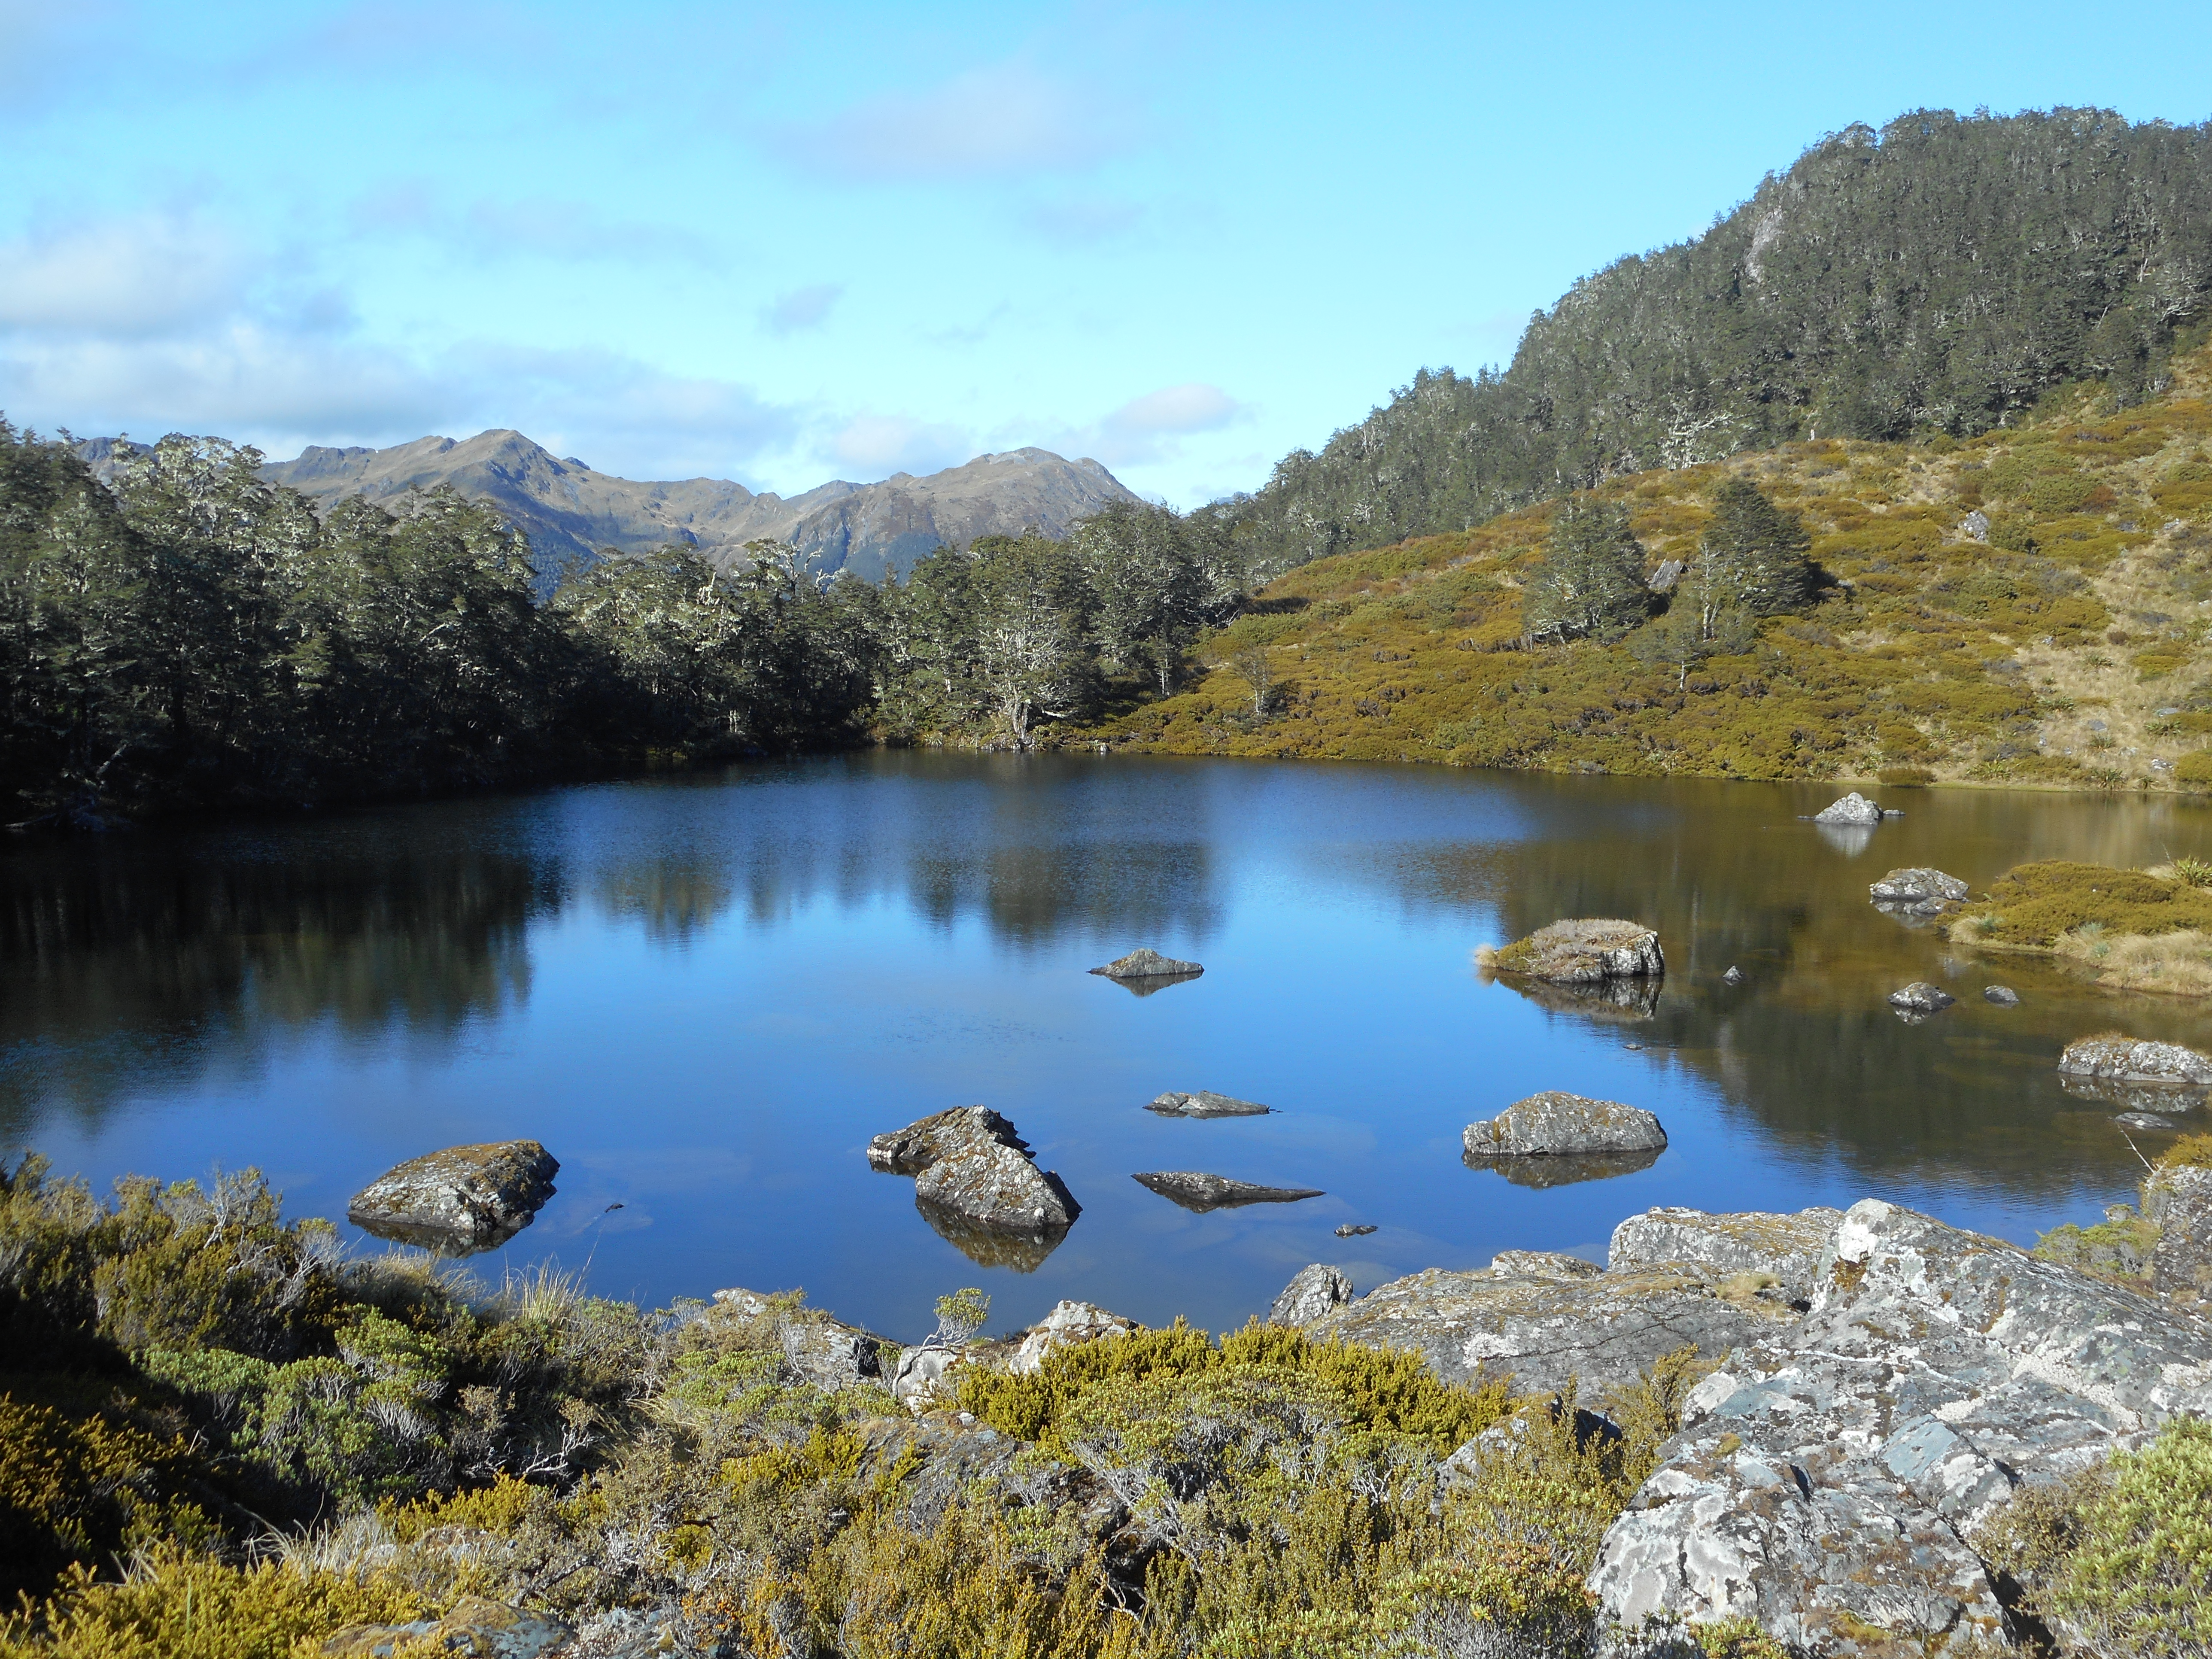
\includegraphics[width=8cm]{MuellerTarn13Nov2017Photo1}
   \captionof{figure}{Mueller Tarn}
\end{flushleft}
\end{minipage}
\begin{minipage}{.5\linewidth}
\begin{flushright}
   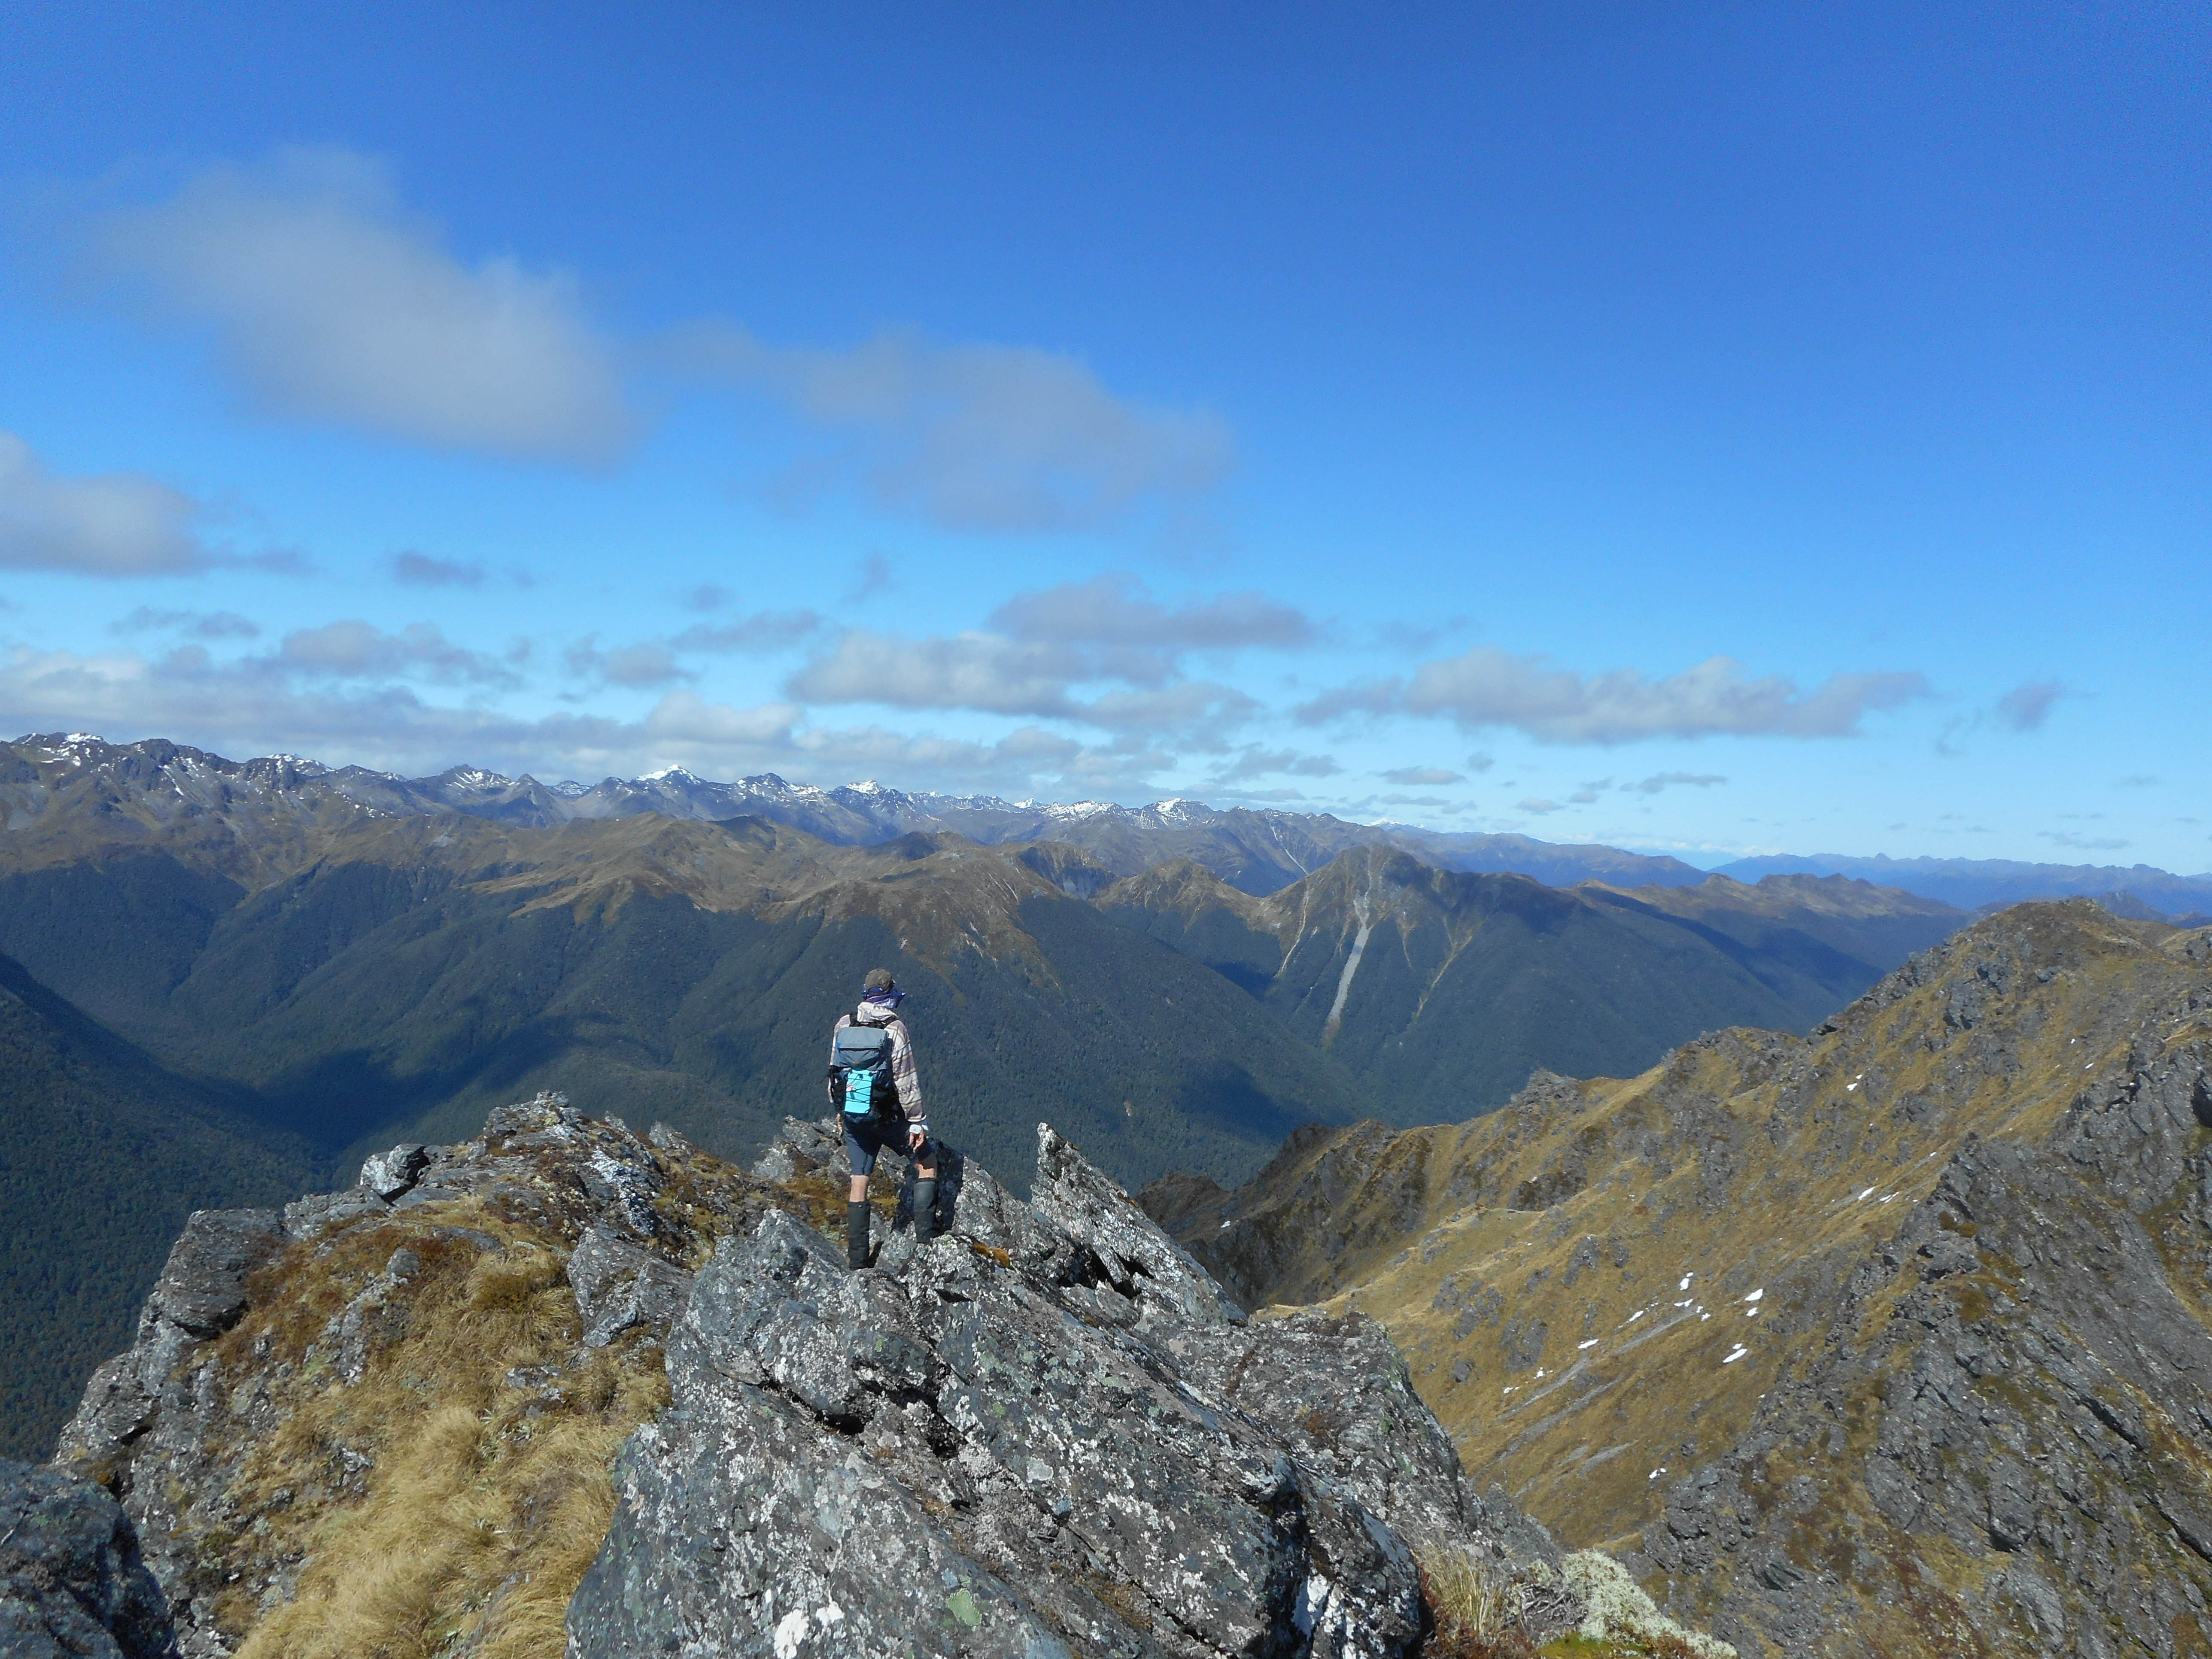
\includegraphics[width=8cm]{MuellerTarn13Nov2017Photo2}
   \captionof{figure}{Looking SW from the top}
\end{flushright}
\end{minipage}
\end{figure}

The following morning we set off after breakfast, heading for a gully leading to the top more or less directly across the tarn.  This looked fairly steep from the camp site, but less so when we were across the the tarn.  However, on actually tackling the gully, it proved to be at least as steep as the first impression.  In fact, Robyn went for a bit of a slide - fortunately doing little damage physically, although tearing her shorts and shaking her confidence.  Once on the ridge, the going was easy.  We climbed to the high point (1566m) and then decided to return along the ridge - all the way this time to approach the camp site from the east.  This was mostly easy going, although a marked track through the final bush section would be useful.

\begin{figure}[ht]
%\centering
\begin{minipage}{.5\linewidth}
\begin{flushleft}
   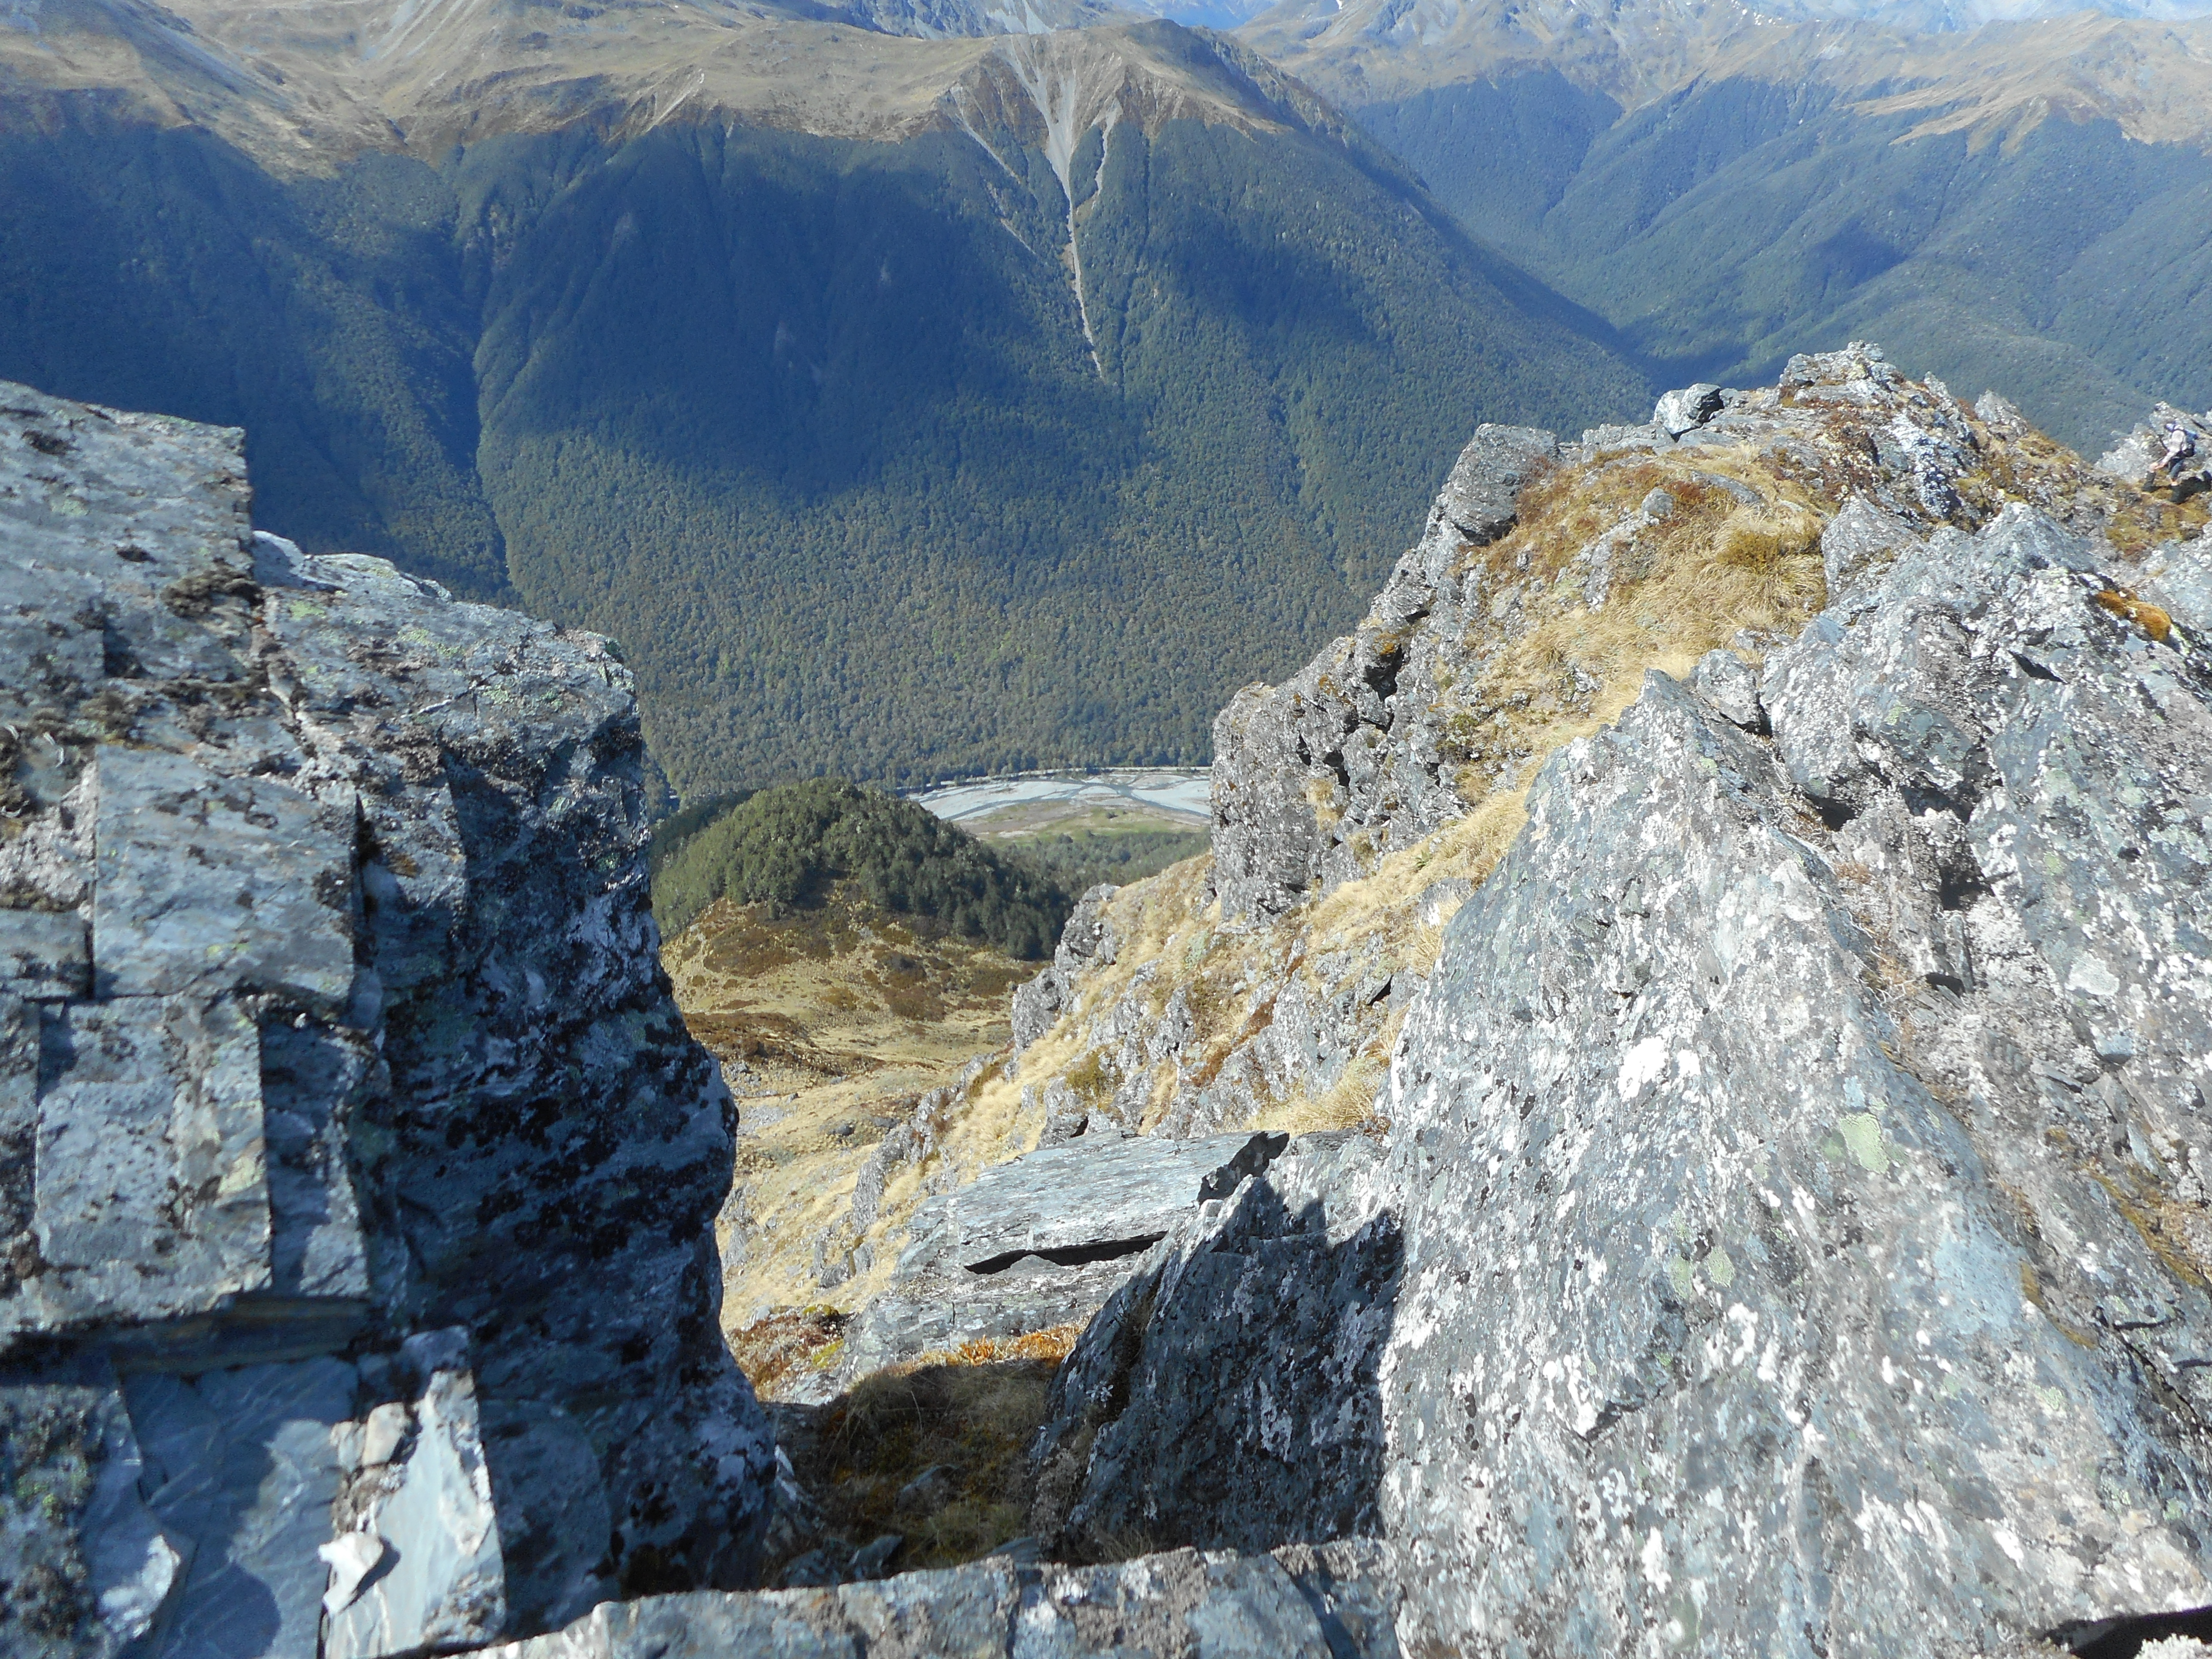
\includegraphics[width=8cm]{MuellerTarn13Nov2017Photo3}
   \captionof{figure}{Braided Maruia River from an ascent gully}
\end{flushleft}
\end{minipage}
\begin{minipage}{.5\linewidth}
\begin{flushright}
   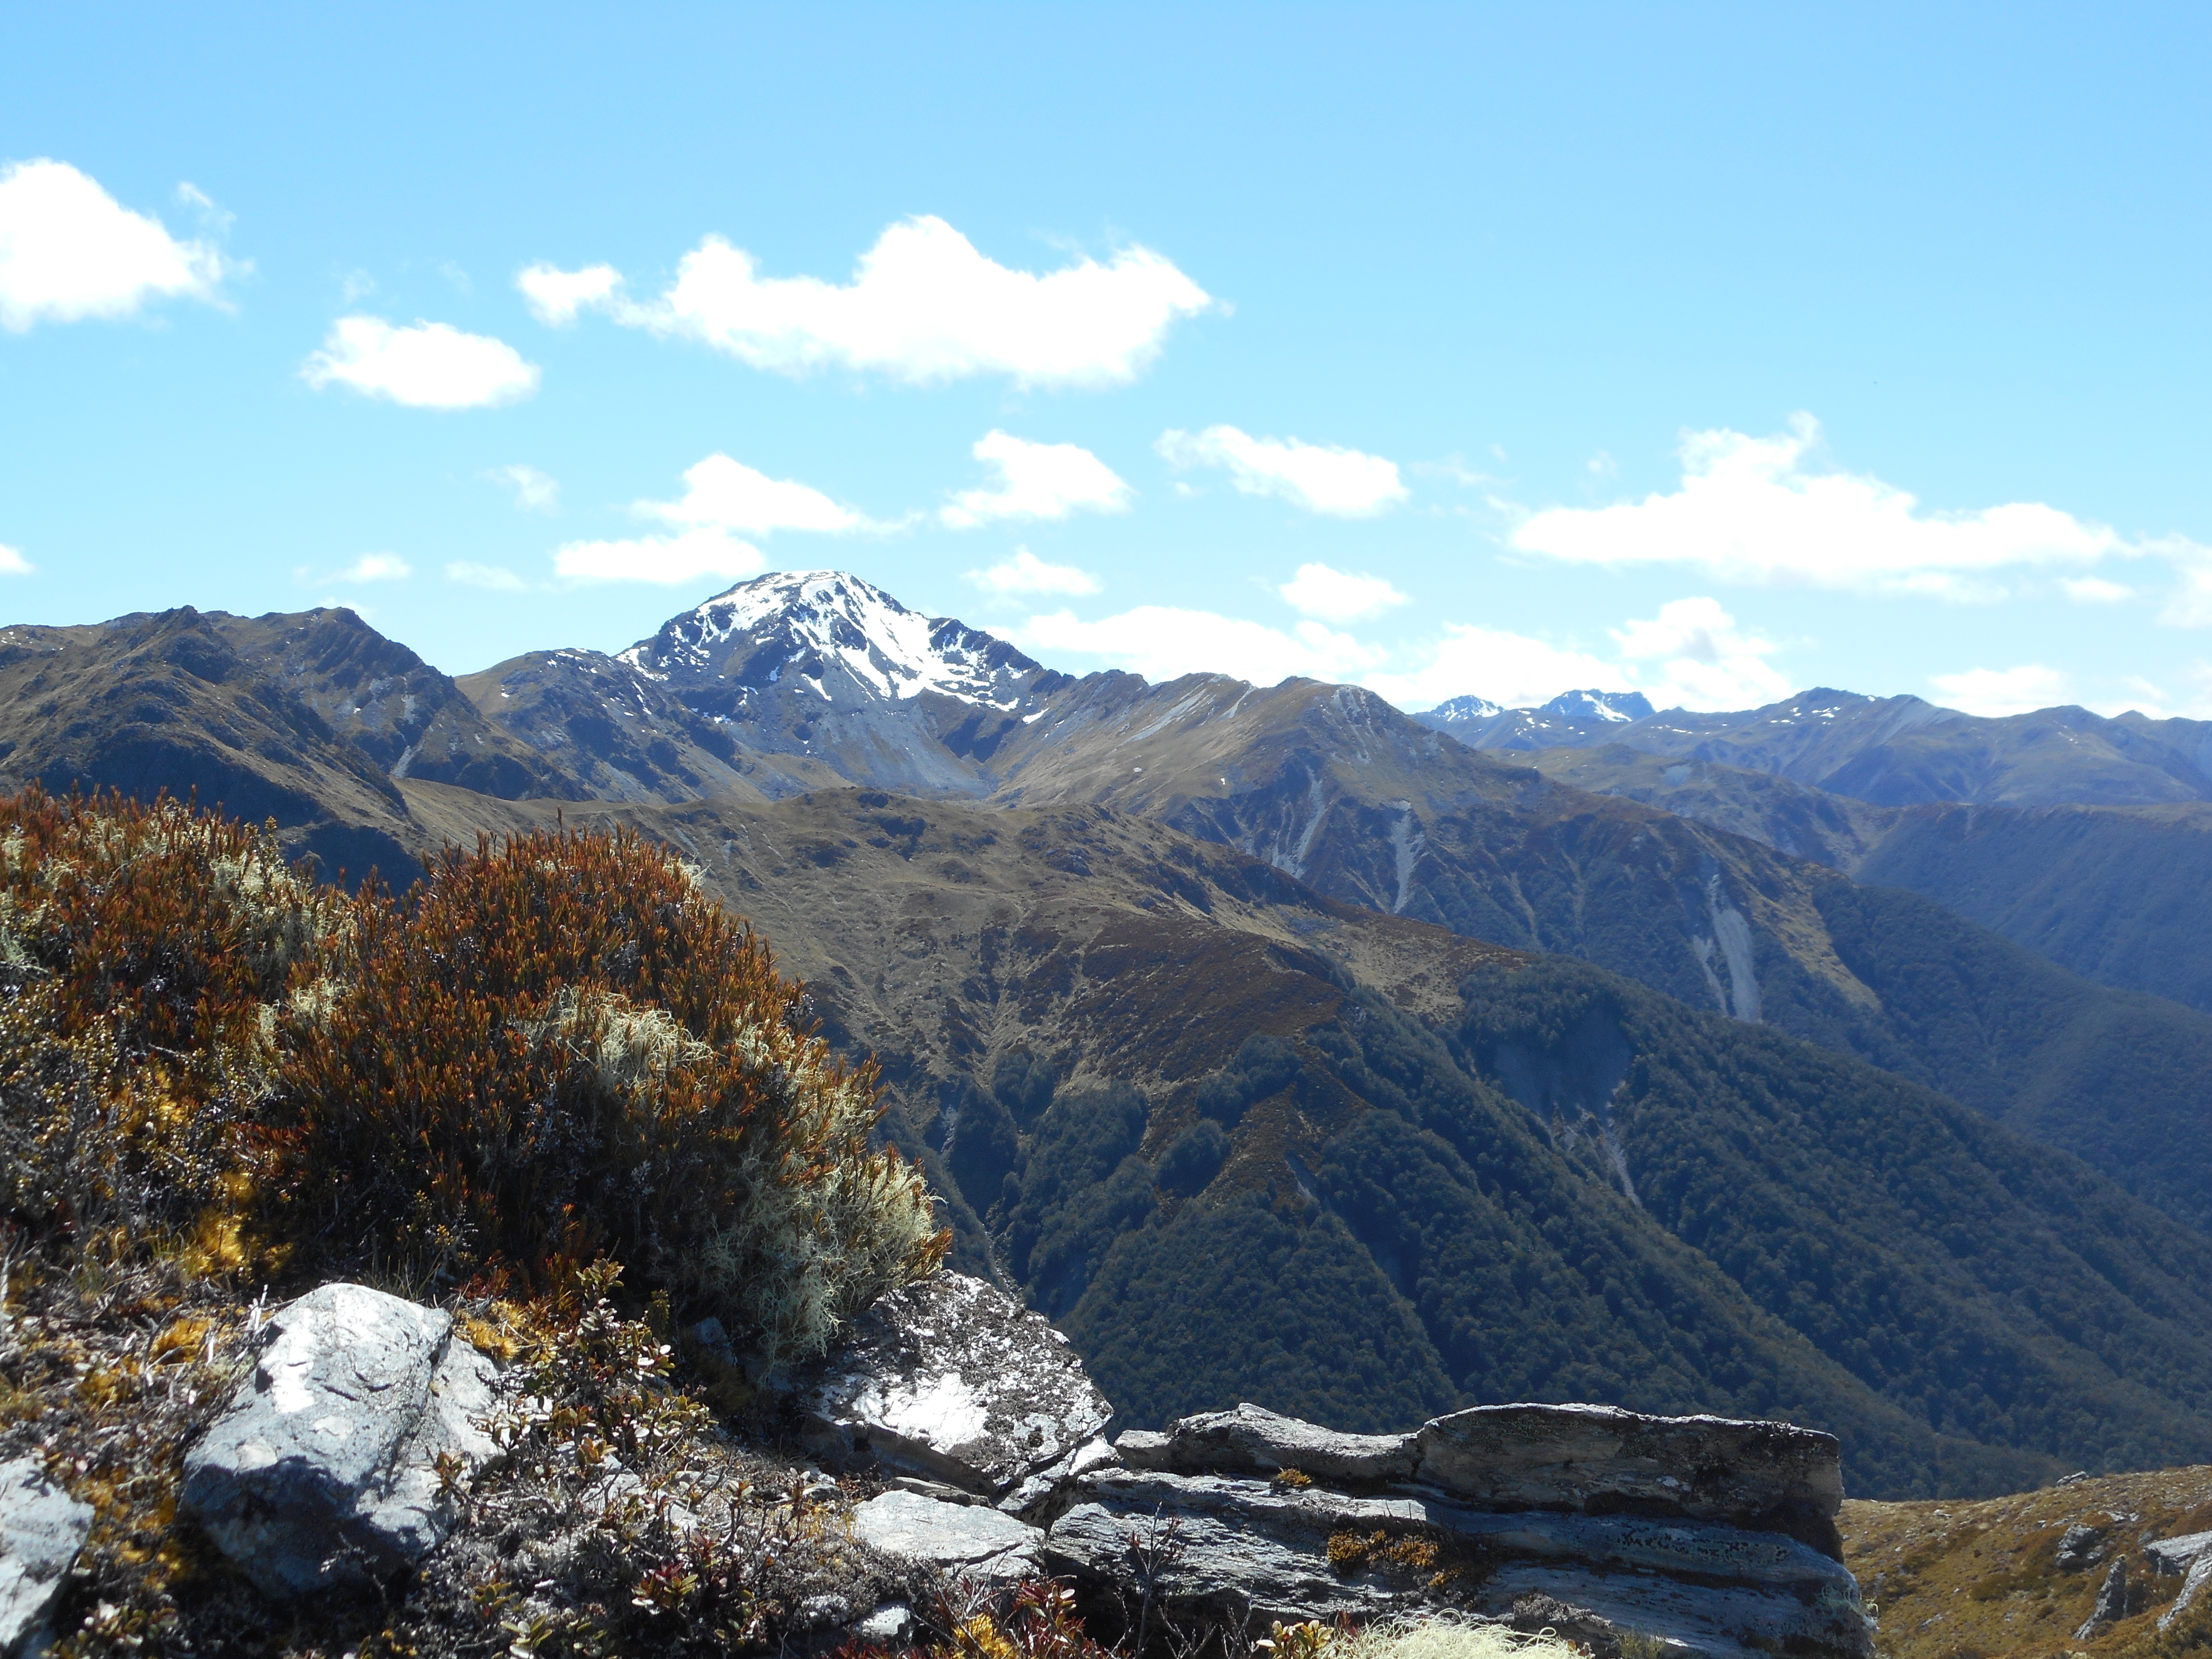
\includegraphics[width=8cm]{MuellerTarn13Nov2017Photo4}
   \captionof{figure}{Mt Freyberg (1816m)}
\end{flushright}
\end{minipage}
\end{figure}

We arrived back in time for lunch.  On the return journey back to the Maruia River, we decided to take the obvious ridge on the true left of the creek just below the first steep section (from the Tarn end).  We had commented before that this looked to be a better route than following the creek, and this proved to be the case.
\begin{flushright}
Robyn, Peter and dog
\end{flushright}

\end{document}
